Como ya se mencionó anteriormente, uno de los principales objetivos de este verificador
 es la posibilidad de extensión para permitir verificar otro tipo de propiedades sobre
 sistemas reactivos.

En esta sección se muestra un ejemplo de extensión para verificar propiedades de
 tiempo real.
Para esto se introducen básicamente los principales conceptos y se describen las
 modificaciones necesarias para verificar este tipo de propiedades.
Esto incluye implementar un lenguaje que
 permita expresar las propiedades deseadas, pero además se necesita modificar la
 estructura de los sistemas de transiciones para modelar el tiempo y así poder expresar
 propiedades teniendo en cuenta el mismo.

\subsection{Sistemas de transiciones con tiempo}
En capítulos anteriores se trabajó con Sistemas de transiciones, pero al momento de verificar
 propiedades de tiempo real estos no permiten modelar el tiempo.
Para poder hacerlo se puede utilizar otro tipo de sistemas de transiciones.
Los sistemas de transiciones con tiempo \cite{henzinger} agregan un conjunto de relojes junto con un
 conjunto de operaciones de comparación y una operación de reinicio.

\begin{definicion}
Sistema de transiciones.\\
Un sistema de trancisiones consiste en una tupla $\text{TS} = (\text{S}, \text{I}, \text{Act}, \text{X}, \text{C}, {\to})$. Donde:
\begin{itemize}
\item $\text{S}$ es el conjunto de estados
\item $\text{I} \subseteq \text{S}$ es el conjunto de estados iniciales
\item $\text{Act}$ es el conjunto de acciones
\item $\text{X}$ es el conjunto de relojes
\item $\text{C}$ es el conjunto comparaciones sobre los relojes
\item ${\to} \subseteq \text{S} \times 2^X \times \text{Act} \times \text{S}$ es la relación de transición
\end{itemize}
\end{definicion}

La definición anterior introduce el conjunto $X$ como el conjunto de las variables
 que modelan los relojes. También introduce el conjunto ${C : S \to {\Phi (X)}}$ de
 comparaciones sobre los relojes. Donde
\[ \Phi (X) = x \leq c | x \geq c | x < c | x > c | \Phi_1 (X) \land \Phi_2 (X) \]
con $c \in \mathbb{R}$.

\paragraph{Ejemplo.} Sistema de transiciones con tiempo para una lámpara\\
Se considera el sistema de transiciones de la figura \ref{fig:lampara} para modelar una
 lámpara. Donde:
\begin{itemize}
\item $\text{S} = \{ \text{apagada}, \text{encendida}_1, \text{encendida}_2 \}$
\item $\text{I} = \{ \text{apagada} \}$
\item $\text{Act} = \{ \text{presionar} \}$
\item $\text{X} = \{ x \}$ 
\item $\text{C} = \{ x < 1 \}$
\item ${\to} = \{ (\text{apagada},\text{presionar},\text{encendida}_1), (\text{encendida}_1,\text{presionar},\text{encendida}_2), (\text{encendida}_1,\text{presionar},\text{apagada}), (\text{encendida}_2,\text{presionar},\text{apagada}) \}$
\end{itemize}

Esta lámpara tiene dos niveles de iluminación, 1 y 2. Para encender la lámpara en el
 modo 2 se debe presionar el botón de encendido dos veces en menos de un segundo.
 
\begin{figure}[hbtp]
\begin{center}
\caption{Sistema de transiciones con tiempo para una lámpara}
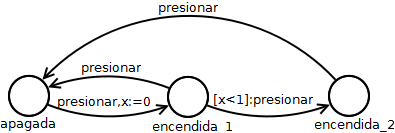
\includegraphics[width=0.5\textwidth]{mc/imagenes/tts.png}
\label{fig:lampara}
\end{center}
\end{figure}


\subsection{Lenguaje de tiempo}
Los lenguajes vistos en capítulos anteriores no permiten expresar propiedades de tiempo
 real, para esto se necesita un lenguaje que incluya variables de tiempo.
Una posibilidad es Lógica Temporal Proposicional de Tiempo (TPTL) \cite{alur}. Este lenguaje es una
 extensión de LTL que permite agregar comparaciones sobre los relojes, las mismas que
 utilizan los sistemas de transiciones con tiempo.
Las fórmulas de TPTL son construídas según la siguiente gramática
\[ \varphi ::= true | a | \varphi \wedge \varphi | \lnot \varphi | \bigcirc \varphi | \square \varphi | \lozenge \varphi | \varphi \cup \varphi | \Phi (X) \]
Donde
\[ \Phi (X) = x \leq c | x \geq c | x < c | x > c | \Phi_1 (X) \land \Phi_2 (X) \]
con $c \in \mathbb{R}$.

\paragraph{Ejemplo.} Propiedades de tiempo para una lámpara\\
A continuación se muestran posibles propiedades en TPTL sobre una lámpara.
\begin{itemize}
\item Si la lámpara está apagada y se presiona dos veces el botón
 de encendido en un tiempo mayor a un segundo, la lámpara se enciende apaga
\[ \lnot ((\text{apagada} \wedge \bigcirc \bigcirc (x \geq 1)) \wedge (\lnot \bigcirc \bigcirc \text{apagada})) \]
\item Si la lámpara está apagada y se presiona dos veces el botón
 de encendido en menos de un segundo, la lámpara se enciende en modo de iluminación 2
\[ \lnot ((\text{apagada} \wedge \bigcirc \bigcirc (x < 1)) \wedge (\lnot \bigcirc \bigcirc \text{encendida}_2)) \]
\end{itemize}


\subsection{Modificaciones en la implementación}
Para implementar los sistemas de transiciones con tiempo se debe agregar una subclase
 de \texttt{TS} con las operaciones necesarias para manipular los relojes.
Ademas se debe implementar una subclase de \texttt{TSTransicion} que incluya las
 guardas y los reinicios de relojes.

Por otro lado para agregar un lenguaje de propiedades es necesario implementar un nuevo
 módulo, incluyendo el parser con la definición de la gramática para este lenguaje.
Este módulo además debe tener una función \texttt{verificar()} que implemente el algoritmo
 de verificación para este lenguaje\footnote{El algoritmo de verificación no se introcuce
 en este documento.}.